\documentclass[10pt,twocolumn,letterpaper]{article}

\usepackage{cvpr}
\usepackage{times}
\usepackage{epsfig}
\usepackage{graphicx}
\usepackage{amsmath}
\usepackage{amssymb}
\usepackage{booktabs}

% Include other packages here, before hyperref.

% If you comment hyperref and then uncomment it, you should delete
% egpaper.aux before re-running latex.  (Or just hit 'q' on the first latex
% run, let it finish, and you should be clear).
\usepackage[breaklinks=true,bookmarks=false]{hyperref}

\cvprfinalcopy % *** Uncomment this line for the final submission

\def\cvprPaperID{****} % *** Enter the CVPR Paper ID here
\def\httilde{\mbox{\tt\raisebox{-.5ex}{\symbol{126}}}}

% Pages are numbered in submission mode, and unnumbered in camera-ready
%\ifcvprfinal\pagestyle{empty}\fi
\setcounter{page}{1}
\begin{document}

%%%%%%%%% TITLE

\title{Modelling and Functional Characterization of the Pyridoxamine Kinase/Phosphomethylpyrimidine Kinase Domain Family}

\author{
Marco Uderzo\\
{\small Department of Mathematics, University of Padua}\\
{\tt\small marco.uderzo@studenti.unipd.it}\\
{\tt\small ID: 2096998} \\
\and
Tanner Graves\\
{\small Department of Mathematics, University of Padua}\\
{\tt\small tanneraaron.graves@studenti.unipd.it}\\
{\tt\small ID: 2073559} \\
\and
Claudio Palmeri \\
{\small Department of Mathematics, University of Padua}\\
{\tt\small claudio.palmeri@studenti.unipd.it}\\
{\tt\small ID: 2062671} \\
}


\maketitle
%\thispagestyle{empty}


%%%%%%%%% ABSTRACT
\begin{abstract}
    This project aims to build a sequence model and provide a comprehensive functional characterization of the Pyridoxamine Kinase/Phosphomethylpyrimidine Kinase domain family. The models' accuracy is benchmarked against Pfam annotations in the SwissProt database. Furthermore, we delved into the functional and structural properties of the domain family, analyzing the taxonomic lineage, assessing Gene Ontology (GO) annotations for functional enrichment, and searching for significantly conserved short motifs inside the family. In particular, our investigation into conserved short motifs using ELM and ProSite databases identified several significant motifs, such as the WDR5 WD40 Repeat-binding ligand and the N-myristoylation site.
\end{abstract}

%%%%%%%%% BODY TEXT
\section{Introduction}

\subsection{Protein Domains}

A \textit{protein domain} represents a conserved part of a protein's sequence and three-dimensional structure, capable of evolving, functioning, and existing independently from the rest of the protein chain. These domains, each forming a stable and compact 3-D structure, are essential components in proteins, often occurring in various combinations across different proteins. Domains are fundamental in molecular evolution, serving as versatile building blocks that can be rearranged to form proteins with diverse functions. This adaptability and independence make them crucial in understanding protein structure and function.

\subsection{Pyridoxamine Kinase / Phosphomethylpyrimidine Kinase}

The \textit{Pyridoxamine Kinase / Phosphomethylpyrimidine Kinase}\cite{family} family is a group of enzymes that play key roles in various biochemical pathways, particularly in the metabolism of vitamins and coenzymes. This family includes two distinct but related enzymes:

\begin{itemize}
\item \textit{Pyridoxamine Kinase}: This enzyme is involved in the vitamin B6 metabolism pathway. Vitamin B6 exists in different forms, including pyridoxamine, pyridoxal, and pyridoxine. Pyridoxamine kinase specifically catalyzes the phosphorylation of pyridoxamine, converting it into pyridoxamine 5'-phosphate. This is an important step in the salvage pathway of vitamin B6, which is crucial for its recycling and maintenance within the cell.

\item \textit{Phosphomethylpyrimidine Kinase}: This enzyme plays a role in the biosynthesis of thiamine (vitamin B1), which is essential for numerous cellular functions, particularly in carbohydrate metabolism.
\end{itemize}

Both these enzymes, due to their roles in vitamin metabolism, are crucial for maintaining cellular health and function. Disruptions in these pathways can lead to vitamin deficiencies, affecting numerous biological processes.

\subsection{Objective of the Study}

In this project, our primary objective is to construct and refine a sequence model for the \textit{Pyridoxamine Kinase/Phosphomethylpyrimidine Kinase} domain family, and to characterize its functional aspects. To ensure the reliability and accuracy of our models, we are aligning and comparing them against the established Pfam annotations within the \textit{SwissProt} database. We then delve into the domain family's functional and structural attributes. This includes a detailed analysis of their taxonomic lineage, providing insights into their evolutionary history and biological diversity. Additionally, we are assessing the Gene Ontology (GO) annotations. This process is crucial for identifying functional enrichment within the family and understanding the broader biological roles these domains play. Furthermore, we are focused on detecting and analyzing significantly conserved short motifs. The identification of these motifs is essential as they often play critical roles in the domain's functional properties and interactions within the cell.

\section{Domain Model Definition}

\subsection{Model Building}

Firstly, we investigated the target family to model - \textit{Pyridoxamine Kinase/Phosphomethylpyrimidine Kinase} - and verified that the provided representative \texttt{A0A0J9X285}\cite{representative_protein} protein sequence, having Pfam domain \texttt{PF08543}, is indeed characteristic of the protein family. 
This was done by retrieving the seed alignment used to generate the HMM defining the Pfam family from \textit{InterPro}, and aligning the representative query sequence to the seed alignment using \textit{JalView}.

The query spans the length of the seed alignment and the gaps opened in the query correspond to low occupancy regions in the seed alignment. This bolstered our confidence that performing a homology search with our query sequence would have been able to return sequences belonging to the \texttt{PF08543} family. This was done by performing a Position-Specific Iterated BLAST (\texit{PSI-BLAST}) search on \textit{SwissProt}. The results were downloaded as a \texttt{.fasta} file and opened in \textit{JalView}, where we added our query sequence as a reference. The FASTA file was aligned with the query sequence using \textit{Clustal Omega}.

The query sequence overlapped the primary conserved regions of the MSA, and the majority of positions outside of the query had very low occupancy, consisting of sequences that were unusually long. The query bounds for the MSA are observed to be reasonable bounds to trim the MSA, so positions outside this range were trimmed from it. \\

Sequences that opened gaps more than a couple residues long were investigated by referencing the BLAST hit corresponding to that sequence. Many of these instances were from Eukaryotes - which is atypical for this family - and were of reasonable quality. Since it is useful to include this information, no sequences reported by BLAST were discarded. \\

The MSA was finalized by removing the query sequence, and it was then processed to generate a \textit{Position-Specific Scoring Matrix (PSSM)} using the command line \texttt{PSI-BLAST} tool, with the \textit{SwissProt} database as the reference. Finally, the \textit{Hidden Markov Model (HMM)} was built using the \texttt{hmmer hmmbuild} command.

\subsection{Model Evaluation}

The PSSM predictions were generated through PSI-BLAST searches against the SwissProt database.
Parallelly, we used hmmer hmmsearch, and the results were parsed to extract alignments between the HMM and sequences in the SwissProt database. It is worth noting that HMM search initially returned far more results than sequences in the family, so we chose an \texttt{E-value} threshold of \(10^{-38}\) that minimizes the false positive proteins identified by the HMM model to good effect.

Both of the models predict regions in sequences corresponding to our family. We evaluated their performance on two levels:
\begin{itemize}
    \item \texit{Protein-level}: are sequences containing the family correctly identified;
    \item \texit{Residue-level}: are the positions within these sequences correctly identified.
\end{itemize}

\subsubsection{PSSM Protein-Level Performance Evaluation}

The protein-level performances of the PSSM model are shown in the table below:

\begin{center}
    \begin{tabular}{lc}
        \toprule
        Metric & Value \\
        \midrule
        Precision & 0.973 \\
        Recall & 0.48 \\
        F1-Score & 0.643 \\
        Balanced Accuracy & 0.740 \\
        MCC & 0.683 \\
        \bottomrule
    \end{tabular}
\end{center} \\ 

\begin{center}
    \small{Table 2.1: PSSM Evaluation at Protein-Level}
\end{center}


\begin{center}
    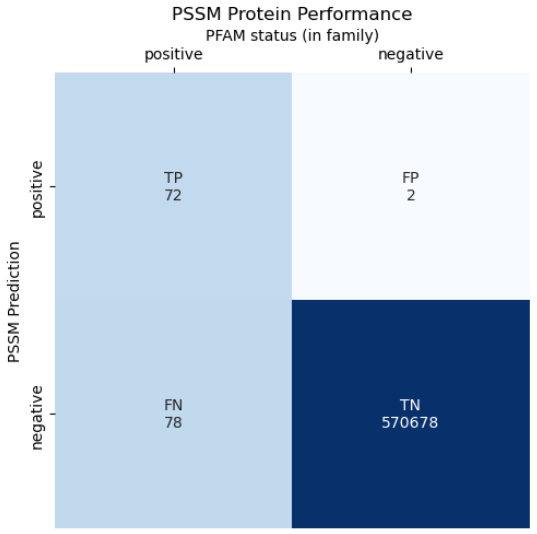
\includegraphics[scale=0.45]{report/img/pssm_prot_performance.png}
\end{center}

\begin{center}
    \small{Fig. 2.1: Confusion Matrix for PSSM at protein-level}
\end{center}

\subsubsection{PSSM Residue-Level Performance Evaluation}

The residue-level performances of the PSSM model are shown in the table below:


\begin{center}
    \begin{tabular}{lc}
        \toprule
        Metric & Value \\
        \midrule
        Precision & 0.980 \\
        Recall & 0.491 \\
        F1-Score & 0.655 \\
        Balanced Accuracy & 0.746 \\
        MCC & 0.694 \\
        \bottomrule
    \end{tabular}
\end{center} \\

\begin{center}
    \small{Table 2.2: PSSM Evaluation at Residue-Level}
\end{center}

\begin{center}
    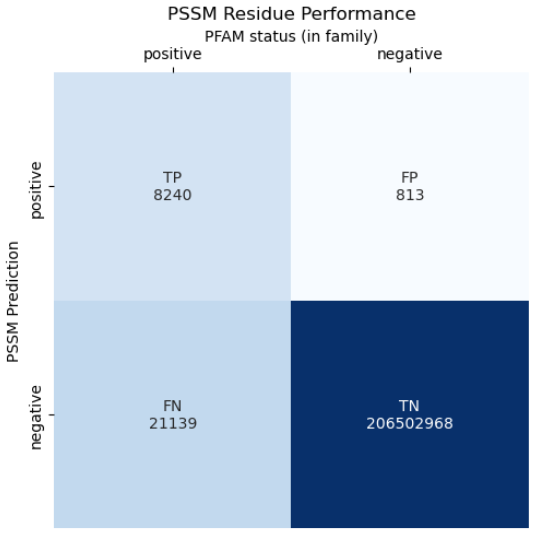
\includegraphics[scale=0.45]{report/img/pssm_res_performance.png}
\end{center}

\begin{center}
    \small{Fig. 2.2: Confusion Matrix for PSSM at residue-level}
\end{center}

\subsubsection{HMM Protein-Level Performance Evaluation}


The protein-level performances of the HMM model are shown in the table below:

\begin{center}
    \begin{tabular}{lc}
        \toprule
        Metric & Value \\
        \midrule
        Precision & 0.993 \\
        Recall & 0.993 \\
        F1-Score & 0.993 \\
        Balanced Accuracy & 0.996 \\
        MCC & 0.993 \\
        \bottomrule
    \end{tabular}
\end{center} \\

\begin{center}
    \small{Table 2.3: HMM Evaluation at Protein-Level}
\end{center}

\begin{center}
    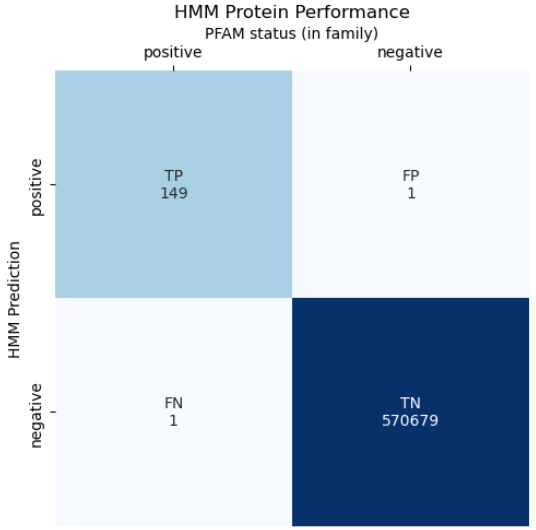
\includegraphics[scale=0.45]{report/img/hmm_prot_performance.png}
\end{center}

\begin{center}
    \small{Fig. 2.3: Confusion Matrix for HMM at protein-level}
\end{center}

\subsubsection{HMM Residue-Level Performance Evaluation}

The residue-level performances of the HMM model are shown in the table below:

\begin{center}
    \begin{tabular}{lc}
        \toprule
        Metric & Value \\
        \midrule
        Precision & 0.989 \\
        Recall & 0.974 \\
        F1-Score & 0.982 \\
        Balanced Accuracy & 0.987 \\
        MCC & 0.982 \\
        \bottomrule
    \end{tabular}
\end{center} \\

\begin{center}
    \small{Table 2.4: HMM Evaluation at Residue-Level}
\end{center}

\begin{center}
    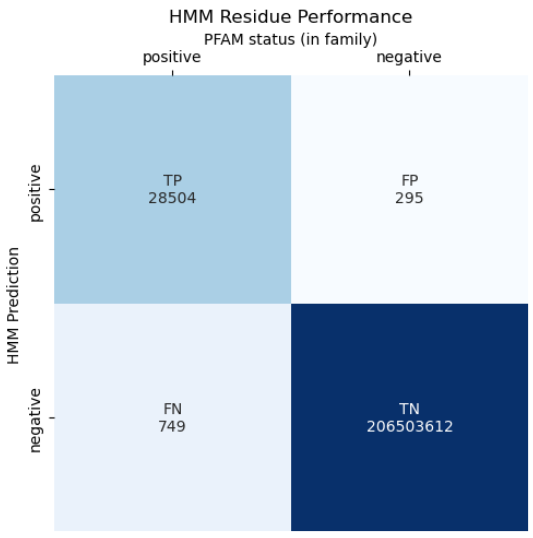
\includegraphics[scale=0.45]{report/img/hmm_res_performance.png}
\end{center}

\begin{center}
    \small{Fig. 2.4: Confusion Matrix for HMM at residue-level}
\end{center}

Both models score very high precision which is due to the fact that the dataset is highly skewed toward negative matches. Only the HMM model is capable of also obtaining a high recall value - and overall much better statistics - thus matching the target PFAM family very closely while the PSSM model only recognizes about half of the target family. Therefore, only the HMM model was used for the next steps of the project.



\section{Domain Family Characterization}

\subsection{Taxonomy}

To construct the taxonomic tree, we assembled the lineage data derived from the \textit{SwissProt} database, corresponding to the proteins identified by our HMM model as belonging to our family. The lineages were used to generate a comprehensive taxonomic tree, which was enriched with node-specific information, including taxonomic names and the frequency of each taxon's occurrence within our data. In our tree, the size of each node indicates how many examples (or leaves) have that taxonomy term. This provides a good visualization of the lineage of taxonomy terms characteristic of our family (i.e. Bacteria, Pseudomonadota, Gammaproteobacteria, Enterobacterales, Enterobacteriaceae, E. coli). \\

The taxonomic tree is shown below. In order to view it in full resolution, we refer to the corresponding \hyperref[sec:taxtree]{section 5.1} in the appendix, or directly to the \texttt{TaxonomyTree.pdf} file that can be found in the supplementary material.

\begin{center}
    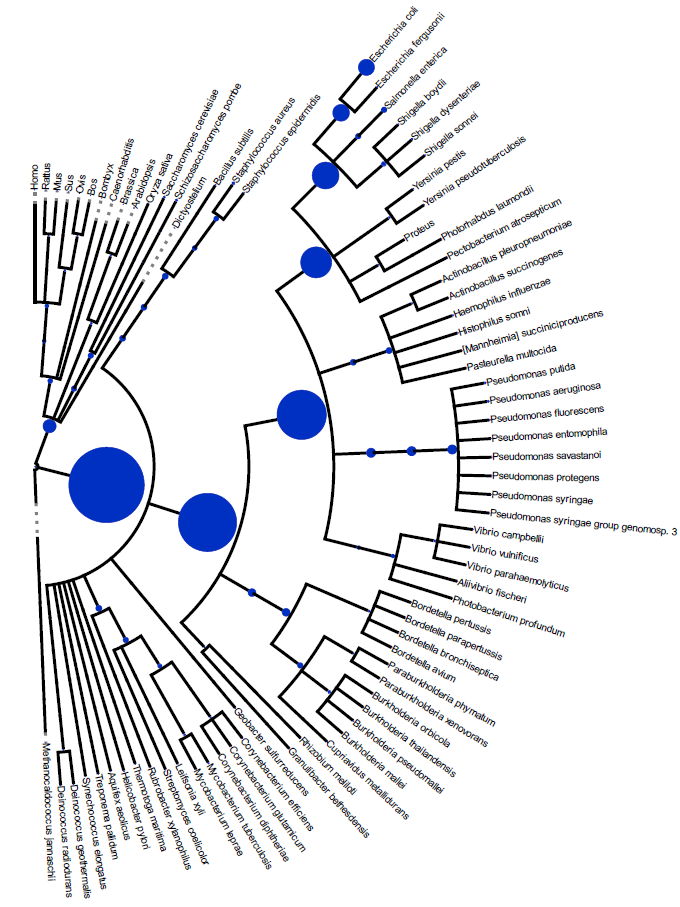
\includegraphics[scale=0.40]{report/img/taxonomy_tree.png}\\
    \small{Fig. 3.1: Taxonomic Tree}
\end{center}

\subsection{Functional Enrichment with Gene Ontology Annotation}

We performed Functional Enrichment Analysis using \textit{Gene Ontology} (GO) annotations by extracting the \textit{molecular function}, \textit{cellular component}, and \textit{biological process} data.

In order to visualize which GO Terms are characteristic of our family, we can plot the enrichment (probability) of observing a GO Term over both our model family and the totality of \textit{SwissProt}. Selecting the terms with the highest odds, or the ratio of probability that the term is observed in the family and all of \textit{SwissProt} gives us clues about which terms are most characteristic. 

\begin{center}
    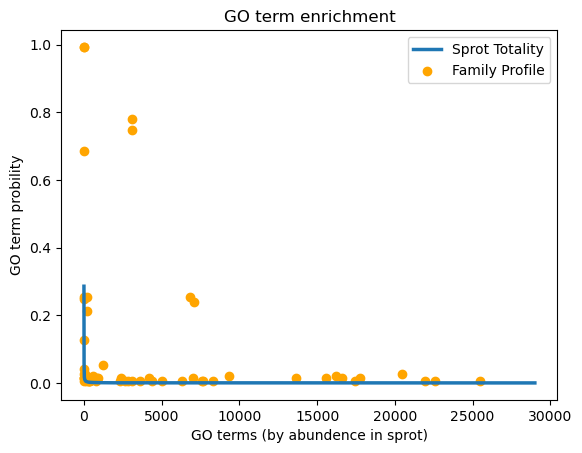
\includegraphics[scale=0.4]{report/img/go_term_enrichment.png}
\end{center}

\begin{center}
    \small{Fig. 3.2: Enrichment of GO Terms}
\end{center}

\begin{center}
    \begin{tabular}{lcc}
        \toprule
        GO Term ID & Term Name & Odds \\
        \midrule
        GO:0042817	& \small{pyridoxal metabolic process} &	3805.53 \\
        GO:0008478	& \small{pyridoxal kinase activity} &	3773.28 \\
        GO:0009443	& \small{pyridoxal 5'-phosphate salvage} &	3642.90 \\
        GO:0008972	& \small{phosphomethylpyrim. kin. act.} &	3615.25 \\
        GO:0008902	& \small{hydroxymethylpyrim. kin. act.} &	3605.24 \\
        GO:0009230	& \small{thiamine catabolic process} &	1902.76 \\
        GO:0042818	& \small{pyridoxamine metabolic process} &	1427.07\\
        GO:0042816	& \small{vitamin B6 metabolic process} &	1268.51\\
        GO:0010054	& \small{trichoblast differentiation} &	1268.51 \\
        GO:0036172	& \small{thiamine salvage} &	1087.29 \\
        GO:0042822	& \small{pyridoxal phosphate metab. proc.} &	951.38 \\
        GO:0070280	& \small{pyridoxal binding} &	845.67 \\
        GO:0031403	& \small{lithium ion binding} &	634.25 \\
        GO:0042819	& \small{vitamin B6 biosynthetic proc.} &	543.64 \\
        GO:0050334	& \small{thiaminase activity} &	456.66 \\
        GO:0097159	& \small{organic cyclic compound binding} &	200.29 \\
        GO:0008614	& \small{pyridoxine metabolic process} &	131.22 \\
        \bottomrule
    \end{tabular}
\end{center} 
\begin{center}
    \small{Table 3.1: Most characteristic GO Terms}
\end{center}

\subsubsection{Fisher's Exact Test}

The Fisher-exact test is useful for testing the nonrandom association between two categorical variables. In our case, possessing a GO term and membership into our family of proteins. In order to conduct the test contingency table for a single GO term of interest must be constructed:
\[
\begin{array}{c|c}
\text{\# in family with term} & \text{\# in family without term} \\ \hline
\text{\# outside fam. with term} & \text{\# outside fam. without term}
\end{array}
\]

The test reporting a low p-value is evidence of the studied GO term being strongly associated with membership in our family. And indeed, we observe that for the terms with the highest odds, the p-value is extremely close to 0. \\


Below, we plot a word cloud of the Enriched Terms for each aspect:

\begin{center}
    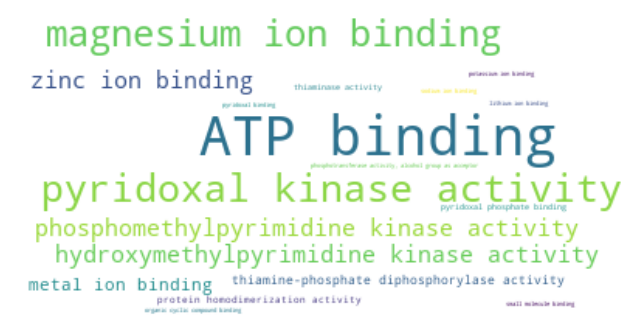
\includegraphics[scale=0.30]{report/img/word_cloud_mf.png} \\
    \
    \small{Fig 3.3: Enriched terms for aspect: Molecular Function}
\end{center}

\begin{center}
    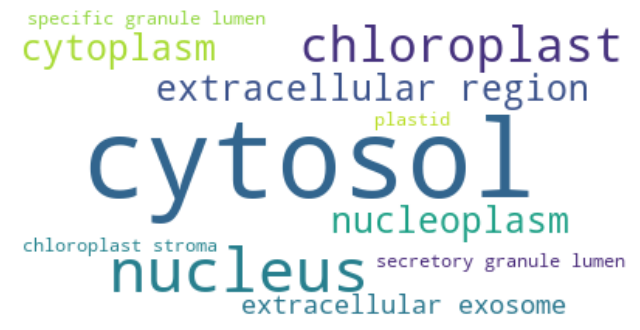
\includegraphics[scale=0.30]{report/img/word_cloud_cc.png} \\
    \
    \small{Fig 3.4: Enriched terms for aspect: Cellular Component}
\end{center}

\begin{center}
    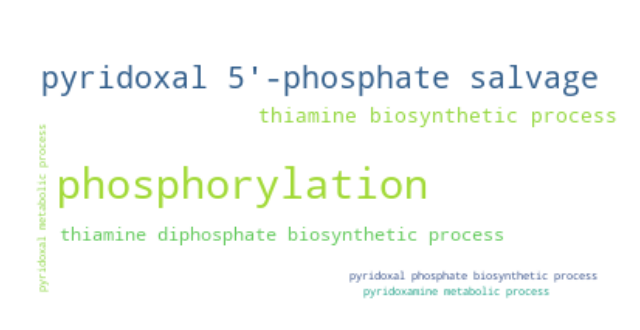
\includegraphics[scale=0.30]{report/img/word_cloud_bp.png} \\
    \
    \small{Fig 3.5: Enriched terms for aspect: Biological Process}
\end{center} \\

We then explored the hierarchical structure of the Gene Ontology to discern the most significantly enriched branches relevant to our protein family. \\

High-level terms in Gene Ontology, typically positioned at the top of the hierarchy, encapsulate the broadest categories, covering a diverse range of specific functions, processes, or components. These general terms are less detailed compared to low-level terms, but are instrumental in offering an overarching view of the primary biological functions, processes, or components linked with a set of genes or proteins. \\

Leveraging the GO hierarchy, each GO Term was classified according to its level of specificity. We focused on high-level terms, filtering the GO terms based on their hierarchical level. This approach enabled us to identify the most enriched branches at a more generalized level, revealing key biological processes, molecular functions, and cellular components prominently involved in our protein family. We report them in the table below:

\begin{center}
    \begin{tabular}{lccc}
        \toprule
        GO Term ID & Term Name & Dom. & Prob. \\
        \midrule
        GO:0005829	& \small{cytosol} & cc & 0.253 \\
        GO:0005576	& \small{extracell. region} & cc & 0.013 \\
        GO:0005654	& \small{nucleoplasm} &	cc & 0.013 \\
        GO:0097159	& \small{org. cyc. comp. binding} & mf	& 0.013 \\
        GO:0036094	& \small{small molecule binding} & mf & 0.013 \\
        \bottomrule
    \end{tabular}
\end{center} 
\begin{center}
    \small{Table 3.2: Most enriched branches}\\
    \small{cc: cellular component; mf: molecular function}\\
    
\end{center}



\subsection{Motifs}
Motifs are short protein sequences that are often repeated across the genome. These motifs usually coordinates protein-to-protein interaction and are found in the disordered regions. \\

Our objective is to see if any commonly occurring linear motifs appear in our \texttt{PF08543} protein family and to do so we have at our disposal two datasets: ELM and ProSite.

For each member of the family we checked if the regular expressions found in the aforementioned two datasets were sub-sequences of it. To do that, we used a precompiled file\cite{prosite_regex} which correlates \textit{ProSite} entries and their corresponding patterns translated to regular expressions. However, the vast majority of the matches found are outside of disordered regions, which can be found with the \textit{MobiDB-lite} database. This is due to the fact that our protein family is constituted by globular proteins.\\

Given a motif, the regions where its pattern matches our proteins are overlayed onto Multiple Sequence Alignments. These patterns are then visually inspected to determine the significance of pattern in the family.
Some patterns are overly general, matching many regions and are labeled as having a high probability of being observed in any given protein sequence from our family.

Conservation of a pattern in the same position is indicative of functional significance.

\subsubsection{ELM}

There were 18 significant hits in the \textit{ELM} Database. Below, we present the most common one.

\paragraph{WDR5 WD40 Repeat (blade 5,6)-binding Ligand}

\begin{center}
    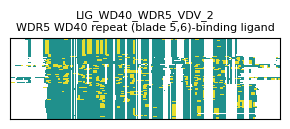
\includegraphics[scale=0.4]{report/img/Elm.png} \\
    \small{Fig 3.7: Most common Elm motif in our family}
\end{center}


The WD40 repeat is a short structural motif, approximately 40 amino acids in length, often terminating in a tryptophan-aspartic acid (W-D) dipeptide. Proteins that contain WD40 repeats are known as WD-repeat proteins. These repeats are typically involved in protein-protein interactions and can form a beta-propeller structure. Each repeat forms a blade of the propeller, with typically 4 to 8 repeats coming together to form a circular propeller-like structure.
WDR5 is a protein containing WD40 repeats, which form a beta-propeller structure, crucial for protein-protein interactions. It plays a pivotal role in the regulation of gene transcription, cell cycle progression, and DNA repair through its involvement in post-translational modifications of histones. Specifically, WDR5 plays a key role in H3K4 methylation and H4K16 acetylation by acting as a scaffold protein for the assembly of the respective core histone methylation and acetylation complex. The WDR5-binding motif, as described by the ELM database \cite{WDR5} (accession \texttt{ELME000365}), is a functional site that interacts with WDR5 between blades 5 and 6 of the WD40 repeat. The WDR5-binding motif is conserved across various species, indicating its importance in biological processes. \\

Plots for the other 17 motifs can be found in the appendix \hyperref[sec:elm_motifs]{section 5.2}. \\

Other common motifs found are:

\begin{itemize}
\item \textit{MOD\_GlcNHglycan}: A Glycosaminoglycan attachment site. 
Glycosaminoglycan are long, linear polysaccharides consisting of repeating disaccharide units. These can be found attached  via a serine residue to proteoglycans which are extracellular proteins found at the cell surface and in the extracellular matrix. The glycosaminoglycan attachment site is an exposed serine which accepts transfer of xylose. \cite{MODGlcNHglycan}
\item \textit{LIG\_FHA\_1}: A FHA phosphopeptide ligand. FHA are small domains that form a sandwich of two anti-parallel beta sheets. The FHA domain is a signal transduction module which recognizes phosphothreonine containing peptides on the ligand proteins and has a role in: cell-cycle checkpoint control, DNA repair, signal transduction, transcriptional regulation, and pre-mRNA splicing.\cite{LIGFHA1}

\item \textit{CLV\_PCSK\_SKI1\_1}: A PCSK cleavage site. 
The subtilisin-like proprotein convertases play a major role in the proteolytic processing of both neuropeptide and peptide hormone precursors.
PCSK1 (proprotein convertase 1) and PCSK2 (proprotein convertase 2) are type I proinsulin-processing enzymes that play a key role in regulating insulin biosynthesis.\cite{CLVPCSKSKI11}

\end{itemize}


It is also worth noting that the \textit{ELM} patterns have identified Casein kinase 1 \& 2 Phosphorylation sites, however they do not appear to be as well preserved than as reported by the ProSite patterns. This can likely be attributed to the ELM patterns being too specific and not accommodating sequence variation in the site, but more investigation is needed.

Also interestingly, many patterns are preserved but may appear in different regions. This is one advantage of plotting the patterns on MSAs, as trying to detect the preservation of these patterns at the position level would miss this.

% \begin{center}
    % \includegraphics[scale=0.4]{report/img/Elm2.png} \\
    % \small{10nth to 18nth most common ELM linear motifs}
% \end{center}

\subsubsection{ProSite}

There were 4 significant hits in the \textit{ProSite} Database. We report the most common one below:

\paragraph{N-myristoylation Site}

\begin{center}
    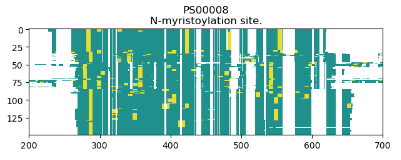
\includegraphics[scale=1]{report/img/prosite.png} \\
    \small{Fig 3.8: Most common ProSite motif in our family}
\end{center}

N-myristoylation consists in the acylation of eukaryotic proteins by the covalent addition to their N-terminal residue of myristate, a C14-saturated fatty acid \cite{N-myristoylation}.
N-myristoylation has been observed happening in animals, plants, fungi, protozoans and viruses. It allows for weak protein–protein and protein–lipid interactions and plays an essential role in membrane targeting, protein–protein interactions and functions widely in a variety of signal transduction pathways, for example in:
\begin{itemize}
    \item \textit{Apoptosis}: The myristoylation of pro-apoptotic BH3-interacting domain death agonist (Bid) leads to the production of cytochrome c which causes cell death.

    \item \textit{Cancer}: Increased myristoylation of c-Src gene can lead to enhanced cell proliferation and be responsible for transforming normal cells into cancer cells
\end{itemize} \\

The other 3 significant hits in the \textit{ProSite} database are the following: 
\begin{itemize}
\item \textit{PS00001}: A N-glycosylation site where oligosaccharides are attached to eukaryotic proteins by binding themselves to the N-terminal asparagine residue.\cite{N-glycosylation}
\item \textit{PS00005}: A protein kinase C phosphorylation site, where protein kinase C manages the phosphorylation of serine or threonine residues near the C-terminal residue.\cite{kinase}
\item \textit{PS00006} A casein kinase II phosphorylation site, where Casein kinase II (CK-2) is a protein serine/threonine kinase whose activity is independent of cyclic nucleotides and calcium. CK-2 functions as a regulator of signal transduction pathways.\cite{kinase2}
\end{itemize} \\

Plots for the top 4 most common motifs in \textit{ProSite} can be found in the appendix at \hyperref[sec:prosite_motifs]{section 5.3}.

\section{Conclusion}

In this project, we have successfully constructed a sequence model for the Pyridoxamine Kinase/Phosphomethylpyrimidine Kinase domain family and provided a detailed functional characterization. Our model, benchmarked against Pfam annotations in the SwissProt database, demonstrated high accuracy in identifying the domain sequences. We analyzed the taxonomic lineage of the domain family, which provided insights into their evolutionary history and diversity. The assessment of Gene Ontology annotations revealed the functional enrichment within the family, highlighting their biological roles and processes.

Additionally, our investigation into conserved short motifs using ELM and ProSite databases was a key aspect of the project. We identified several significant motifs, such as the WDR5 WD40 Repeat-binding ligand and the N-myristoylation site.


%-------------------------------------------------------------------------

{\small
\bibliographystyle{unsrt}
\bibliography{egbib}
}

\clearpage % Start a new page
\onecolumn % Switch to one-column layout

\section{Appendix}


\subsection{Taxonomic Tree}
\label{sec:taxtree}

Below, we plot the full-resolution Taxonomic Tree. \\
\begin{center}
    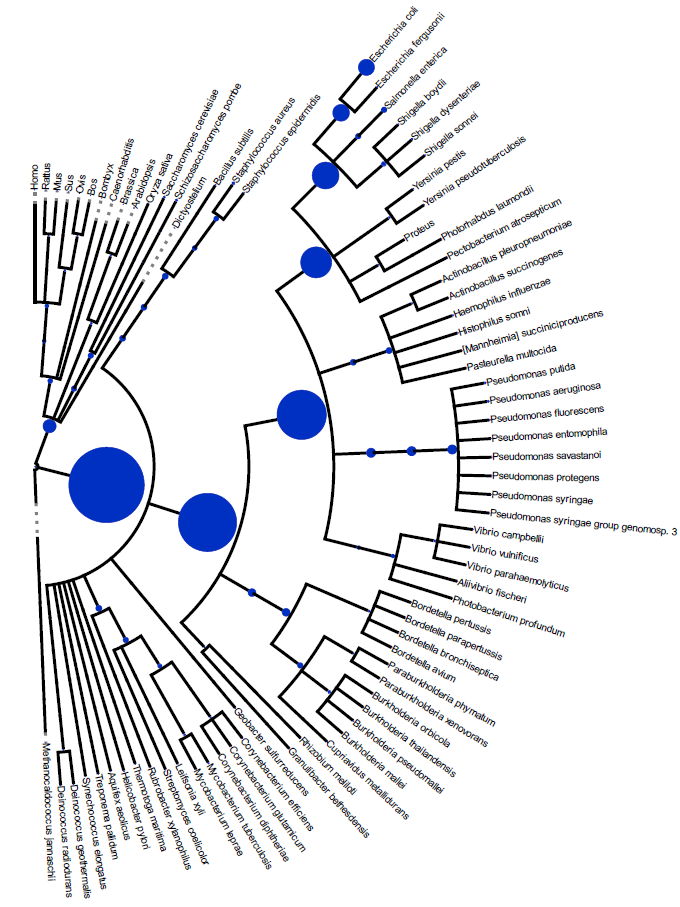
\includegraphics[]{report/img/taxonomy_tree.png}
\end{center}

\subsection{ELM}

Below, we plot the top 9 most common ELM Linear Motifs. \\

\label{sec:elm_motifs}
\begin{center}
    \includegraphics[scale=0.8]{report/img/Elm1.png} \\
    \small{Top 9 most common ELM linear motifs}
\end{center}
\begin{center}
    \includegraphics[scale=0.8]{report/img/Elm2.png} \\
    \small{10th to 18th most common ELM linear motifs}
\end{center}

\newpage
\subsection{ProSite}
\label{sec:prosite_motifs}

Below, we plot the top 4 most common ProSite Linear Motifs. \\

\begin{center}
    \includegraphics[scale=0.58]{report/img/Prosite.png} \\
    \small{Most common 4 ProSite linear motifs}
\end{center}
\end{document}
